\subsection*{Results to date (3.5 months)}

\begin{center}
\colorbox{green!10}{
  \begin{minipage}[t]{0.9\columnwidth}
    \textbf{Summary of completed tasks (3.5 Months):}
      \begin{itemize}[leftmargin=0.5cm]
        \itemsep-0.5em
	\item Identified specific ATM problem, deconflicting trajectories, as case study
        \item Devised code to analyze and visualize wind-optimal trajectories
        \item Identified and characterized all potential conflicts in NAT dataset
        \item Developed formulations of a simpler version of the problem 
with only origination delays, amenable being run on a quantum annealer. Write-up available
        \item Began developing formulations that support manoevers as well
as delays
	\item Identified subsets of data treatable independently, a
first step in the design of a set of small benchmark problems
      \end{itemize}
 \end{minipage}
}
\end{center}


We have identified a specific ATM domain to serve as a case study, 
namely deconflicting wind-optimal aircraft trajectories. We build on
the work of Rodionova et al.~\cite{rodionova:16, rodionova:thesis15}
who developed a non-quantum approach to this problem. The following
graphic shows the main steps in developing a quantum annealing approach 
to these problems. 
\begin{minipage}[c]{\columnwidth}
\centering
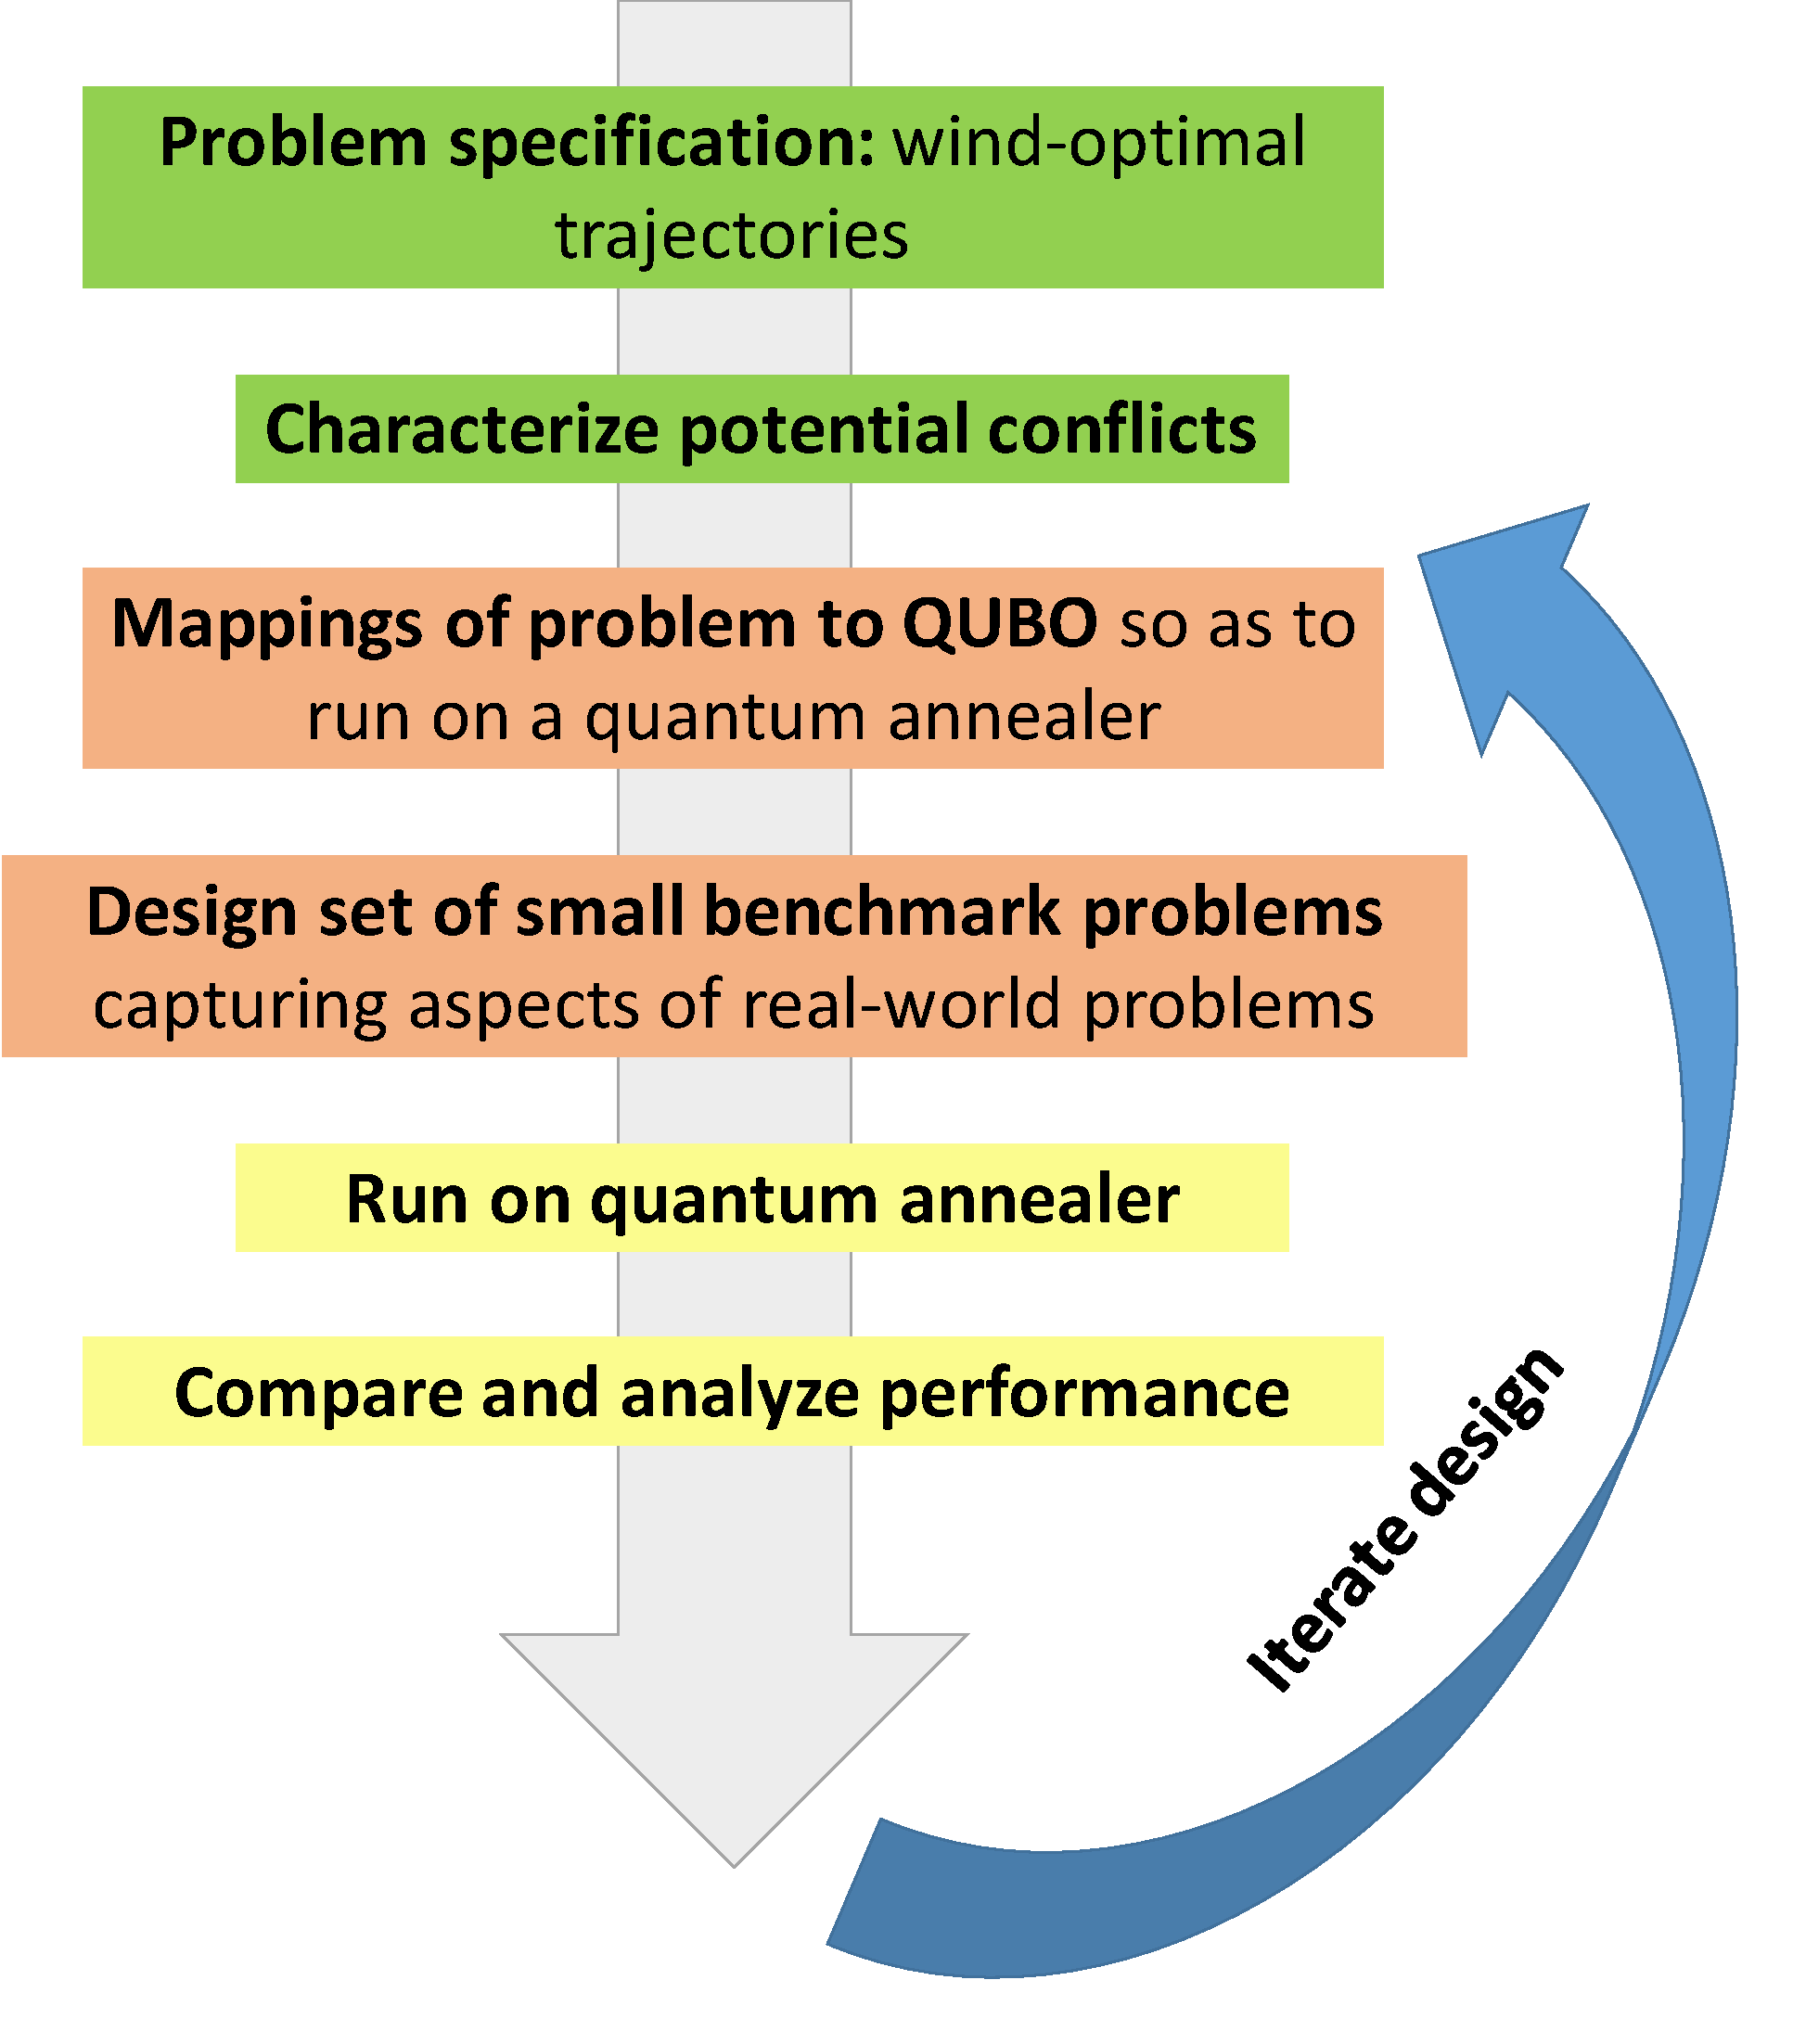
\includegraphics[width=0.8\columnwidth]{flowDiagram}
% \captionof{figure}{Schematic flow diagram to optimize ATM problems using quantum optimizers. Green/light-gray and orange/dark-gray boxes represent respectively completed and partially completed tasks.}
\label{fig:scheme}
\end{minipage}
Throughout this document, green indicates steps
completed in the past 3.5 months, yellow/orange
indicate steps to be completed in the next 4 month period, with orange 
for already partially completed tasks. 
% Uncolored items will be completed within the final 4.5 month stage of the project.

We have formulated a basic version of the problem, one that considers only
origination delays, in a way that is amenable
to quantum computing. Furthermore, we have developed tools to 
characterize the potential
conflicts in order to devise parameterizations and encodings 
of manoevers in flight so that our approach can support quantum annealing
approaches that consider manoevers as well as delays. 
From these formulations, we have developed multiple mappings to 
quadratic unconstrained binary optimization (QUBO), the type of problem
specification current annealers such as the \DW\ require. 

In order to optimize our formulation of the problem for realistic data, we focus
on flight data in the North Atlantic oceanic airspace (NAT). 
Rodionova provided us with
wind-optimal trajectories for two consecutive days (July
28\textsuperscript{th}-29\textsuperscript{th} 2012), trajectories on which her
state-of-the-art approach has been evaluated. 
We have already implemented the first step in processing the raw data
into useful form: given the trajectories, find the set of potential 
conflicts.
We have also developed code to evaluate the dependencies in the data set,
enabling the identification of subsets of the data that can
be treated independently, a step toward the design of suitably small 
benchmark sets that will fit on the \DW\ prototype quantum annealer in spite
of its limitations in terms of number of qubits and connectivity.
